\documentclass{article}
\usepackage[utf8]{inputenc}
\usepackage{geometry}
 \geometry{
 a4paper,
 total={170mm,257mm},
 left=20mm,
 top=20mm,
 }
\usepackage{graphicx}
\graphicspath{ {./plots/} }
\usepackage{caption}
\usepackage{subcaption}
\usepackage{hyperref}

\title{Tennis Matches}

\begin{document}

\begin{titlepage}
    
    \begin{center}
        \vspace*{1cm}
            
        \Huge
        \textbf{Analysis of Tennis Matches Dataset}
            
        \vspace{0.5cm}
        \LARGE
        Data Mining Project
            
        \vspace{1.5cm}
            
        Jacopo Bandoni\\
        Alex Colucci\\
        Domenico Romano\\
            
        \vfill
            
        
\includegraphics[width = 450 px]{logo_unipi.png}
        
        %\vspace{0.5cm}
            
            
        \Large
        Dipartimento di Informatica\\
        Università di Pisa\\
        05/01/2022
            
    \end{center}
\end{titlepage}    

%\maketitle
\tableofcontents
\newpage

% TODO 
% - DATA understanding\\
% - SCRIVERE\\
% - DATA CLEANING\\
% - INDIVIDUARE PROBLEMI E PROPORRE POSSIBILI SOLUZIONI\\



\section{Introduction}

\section{Data understanding}
The \texttt{tennis\_matches} dataset contains $186128$ total observations. Below, the detailed analysis for each individual attribute.

\paragraph{tourney\_id}
The identifier of the tourney. On 185764 observations, there are 4854 unique tourneys and 55 missing.

\paragraph{tourney\_name}
The name of the tourney. On 185794 observations, there are 2488 unique names and 25 missing. The unique values are lower than those of tourney\_id, hence more tournaments with the same name have been played over the years. Moreover, several naming conventions are used from which partial information about the host city name, prize, nationalities could be scraped.

\paragraph{surface}
The type of surface on which the players had the game. On 185793 observations, 26 are missing. The types are the following with their respective occurrences: Hard (95127), Clay (81013), Grass (6600), Carpet (3053).

\paragraph{draw\_size}
The number of players in the draw, that is often rounded up to the next power of $2$. The most common draw size for a tourney is $32$ followed by $2,4,64$.

\paragraph{tourney\_level}
The level of the tourney that is different for men and women, and hence it gives information about the sex of a tournament. On 185790 observations 19 are unique and 25 are missing. They are mostly character, but for ITF competitions it's an integer that states the prize. The only ambiguous level is the $D$ that is used both for men and women, but it can be disambiguated thanks to the fact that for men it's used only in the tourney whose name are “Davis Cup F.” Moreover, $O$ is a category used to denote the Olympics, where both men and women can participate. 

\paragraph{tourney\_date}
The date when the tourney started. On 185791 observations of which $28$ are missing.
The matches were disputed between the year $2016$ and $2021$, with most of them in the range $2016-2019$. For the months, instead, November and December tends to be the one with fewer matches. More than 97\% of them are on Monday.

\paragraph{match\_num}
A match-specific identifier. Often starting from 1, sometimes counting
down from 300, and sometimes arbitrary. On $186103$ observations, $27$ are missing.

\paragraph{winner\_id, loser\_id}
The player\_id used in this repo for the winner/loser of the match. On $186103$ observations, $55$ for the winners and $28$ for the losers are missing.

\paragraph{winner\_entry, loser\_entry}
The player\_id used in this repo for the winner/loser of the match. On $186103$ observations, $160008$ for the winners and $141731$ for the losers are missing.

\paragraph{winner\_hand, loser\_hand}
The hand used by the player. For ambidextrous players, this is their serving hand. On $186103$ observations, $46$ for the winners and $98$ for the losers are missing. A possible value for those attributes is 'U' which stands for unknown, and it matches $49k$ and $62k$ for winners and losers respectively.

\paragraph{winner\_name, loser\_name}
Winner's/loser's name. On $186103$ observations, $27$ for the winners and $31$ for the losers are missing.

\paragraph{winner\_ht, loser\_ht}
Winner's/loser's height in centimetres. On $186103$ observations, $136516$ for the winners and $147489$ for the losers are missing.

\paragraph{winner\_ioc, loser\_ioc}
Winner's/loser's three-character country code. On $186103$ observations, $29$ for the winners and $26$ for the losers are missing.

\paragraph{winner\_age, loser\_age}
Winner's/loser's age, in years, depending on the date of the tournament. On $186103$ observations, $2853$ for the winners and $6537$ for the losers are missing.

\paragraph{round}
An acronym which identifies the stage of the match inside the tournament (e.g., 'f' stands for 'final', 'sf' for 'semifinal' and so on).

\paragraph{score}
The score of the match. On $186103$ observations, $175$ are missing. 
Every couple n1-n2 (e.g., 6-4) represents the score of a single set, where n1 are the games won by the winner and n2 those won by the loser of the match.
When after the couple of numbers representing a set there is a number n3 between brackets (e.g., 7-6(4)), it means that the set ended at the tie-break and n3 represents the points scored during it by the loser of the set.
When we find a couple between square brackets (e.g., [10-7]), it represents the result of the super tie-break, which is played in some tourneys, on the 6-6 of the last set (on the 12-12 in Wimbledon). In these cases, the score of the final set is omitted.
We can also find some abbreviations, which indicate particular conditions:
\begin{itemize}
    \item \verb|RET, Ret., RE, RET+64|. Placed at the end of the score, to indicate the retirement of a player during the match.
    \item \verb|W/O, Walkover|. It's the retirement of a player before the match starts. 
    \item \verb|DEF, Def.|. It's a default, i.e., the disqualification of a player.
    \item \verb|BYE|. It's the automatic advancement of a player to the next round of a tournament without facing an opponent. 
\end{itemize}
Furthermore, there are some errors: not recognized characters (16 times), HTML non-breaking spaces (15), “RET” without a score before (8), "2-May", "1-Feb" and a score with a wrong formatting.

\paragraph{best-of}
The maximum number of sets of the match. If "3", it means that the first player to achieve 2 sets, wins the match. If "5", a player must achieve 3 sets to win.  On $186103$ observations, $0$ are missing.

\paragraph{minutes}
The duration of the match. On $186103$ observations, $104461$ are missing.

\paragraph{w\_ace, l\_ace}
Winner's/loser's number of aces. On $186103$ observations, $103811$ for the winners and $103808$ for the losers are missing.

\paragraph{w\_df, l\_df}
Winner's/loser's number of double faults. On $186103$ observations, $103809$ for the winners and $103802$ for the losers are missing.

\paragraph{w\_svpt, l\_svpt}
Winner's/loser's number of serve points. On $186103$ observations, $103811$ for the winners and $103806$ for the losers are missing.

\paragraph{w\_1stIn, l\_1stIn}
Winner's/loser's number of first serves made. On $186103$ observations, $103811$ for the winners and $103817$ for the losers are missing.

\paragraph{w\_1stWon, l\_1stWon}
Winner's/loser's number of first-serve points won. On $186103$ observations, $103809$ for the winners and $103810$ for the losers are missing.

\paragraph{w\_2ndWon, l\_2ndWon}
Winner's/loser's number of second-serve points won. On $186103$ observations, $103812$ for the winners and $103809$ for the losers are missing.

\paragraph{w\_SvGms, l\_SvGms}
Winner's/loser's number of serve games. On $186103$ observations, $103810$ for the winners and $103803$ for the losers are missing.

\paragraph{w\_bpSaved, l\_bpSaved}
Winner's/loser's number of breakpoints saved. On $186103$ observations, $103806$ for the winners and $103810$ for the losers are missing.

\paragraph{w\_bpFaced, l\_bpFaced}
Winner's/loser's number of breakpoints faced. On $186103$ observations, $103809$ for the winners and $103815$ for the losers are missing.

\paragraph{winner\_rank, loser\_rank}
Winner's/loser's ATP or WTA rank, as of the tourney\_date, or the most recent ranking date before the tourney\_date. On $186103$ observations, $19402$ for the winners and $35259$ for the losers are missing.

\paragraph{winner\_rank\_points, loser\_rank\_points}
Number of ranking points. On $186103$ observations, $19420$ for the winners and $35276$ for the losers are missing.

\paragraph{tourney\_spectators}
The number of total spectators of the tourney. On $186103$ observations, $27$ are missing.

\paragraph{tourney\_revenue}
The total tournament earnings. On $186103$ observations, $26$ are missing.

\section{Data cleaning and transformation}

First we switched all the letters in lowercase, since in some cases there were equivalent values considered as different (e.g., “US Open” and “Us Open” in tourney\_name), we also removed double spaces where present because they could lead as well into the same kind of problems. Then we applied the following changes:

\paragraph{score}
We set to NaN all the erroneous values. We also added the omitted final set score in the matches with super tie-break, in order to be able to compute the number of games won by the winner and those won by the loser. Lastly, we uniformed the different strings that represented the same concept (e.g., “w/o” and “walkover”).

\paragraph{minutes}
This attribute was full of outliers. In particular, we noticed that all the values grater than 396 were not possible, also in relation to the score of the matches. So we substituted these values with NaN.

\paragraph{winner\_ht}
Several outliers with winner\_ht = 2.0 and also other outliers with height < 146. In this case, we decide to search on the internet the correct values and replace those with the outliers.

\paragraph{winner\_ht}
Several outliers with loser\_ht = 2.0, even in this case we decide to search on the internet the correct values and replace those with the outliers.

\paragraph{winner\_age}
There were two players with two occurrences having as winner\_age 95 years. Then we decide to replace those values with the medium age of the corresponding players.

\paragraph{w\_svpt, w\_1stIn, w\_1stWon, w\_2ndWon and corresponding of the loser}
We noticed that for all these attributes there were 5 recurrent records in which the values were extremely high and not possible, also in relation to the score of the matches. We dropped these records.

\paragraph{gender}
For each player where the gender was missing, we replace that gender by checking in all his game the most frequent gender's opponent.

\section{Players dataset}

\subsection{Feature engineering}

\paragraph{matches\_won\_ratio}
The ratio between the number of the total games won and the total numbers of games played.

\paragraph{mean\_performance\_index, max\_performance\_index, min\_performance\_index }
The minimum, the maximum and the average value of the performance index, which is the ratio between the number of matches played by the player in a tourney and the number of matches he should have played in order to win the tourney.

\paragraph{mean\_minutes, max\_minutes, minutes\_entropy }
The average, the maximum, and the Shannon entropy of the duration of the matches played by a player.

\paragraph{rel\_ace, rel\_df, rel\_1stIn, rel\_1stWon, rel\_2ndWon}
The average of the ratios between the statistics (ace, df etc.) and the number of serve points of the player in the single matches.

\paragraph{1stWonOnTotWon}
The average of the ratios between the first serve point won and player's total serve points in the single matches.

\paragraph{2ndWonOnTotWon}
The average of the ratios between the second serve point won and the total points won by the player in the single matches.

\paragraph{rel\_bpFaced}
The average of the ratios between the breakpoints faced and the player's total serve points in the single matches.

\paragraph{rel\_bpSaved}
The average of the ratios between the breakpoints saved, and the breakpoint faced by the player in the single matches.

\paragraph{rel\_ptsWon}
The average of the ratios between the points scored and the total by the player in the single matches.

\paragraph{rel\_gmsWon}
The average of the ratios between the breakpoints saved, and the breakpoint faced by the player in the single matches.

\paragraph{lrpOnAvgrp}
The ratio between the player's last ranking points (last\_rank\_points) and his average ones (mean\_rank\_points).

\paragraph{lrpOnMxrp}
The ratio between the player's last ranking points (last\_rank\_points) and the maximum ones he ever achieved (max\_rank\_points).

\paragraph{Other trivial features}
name, gender, ht, age, hand, total\_tourneys\_played, total\_matches\_played,\\ total\_matches\_won, last\_rank\_points, mean\_rank\_points, max\_rank\_points, variance\_rank\_points, \\ mean\_tourney\_spectators, max\_tourney\_spectators, mean\_tourney\_revenue, max\_tourney\_revenue.    
\newpage
\section{Clustering}
Since in the player's dataframe there was a big number of records with NaN values, corresponding to the in-match statistics (rel\_ace, rel\_df, rel\_1stIn etc.), we set a threshold establishing that every player in order to be in the dataframe should have played at list 15 matches with non-null values for these features.
Then we selected the features which seemed to better represent the “strength” of a player, and we performed the correlation analysis (Fig. \ref{fig:correlation_plot}) in order to have a narrower selection. Whenever two features had a correlation greater than 70\% (Pearson coefficient), we discarded one of the two. 
\begin{center}
    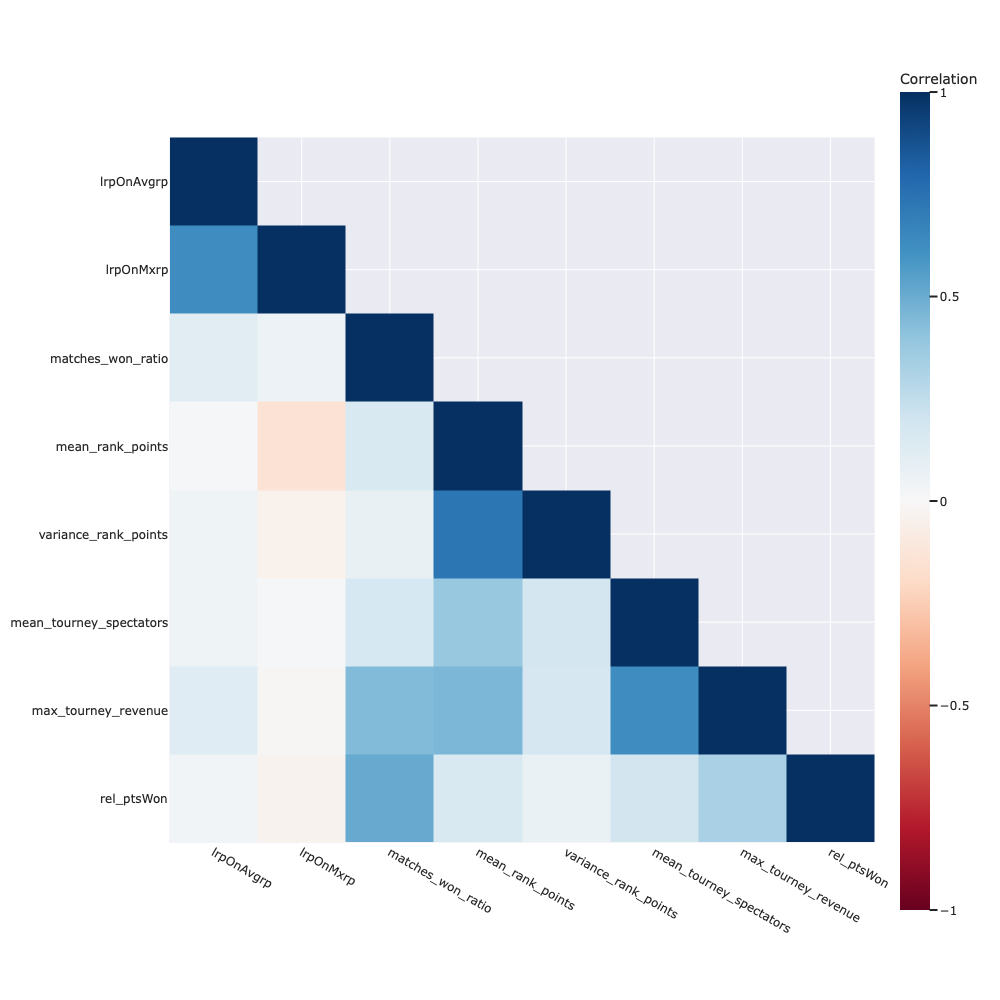
\includegraphics[width=350px]{correlation_plot}
    \label{fig:correlation_plot}
    \captionof{figure}{Correlation plot of the selected features}
\end{center}
At this point the remaining features were: 'lrpOnAvgrp', 'lrpOnMxrp', 'matches\_won\_ratio', 'mean\_rank\_points', 'variance\_rank\_points', 'mean\_tourney\_spectators', 'max\_tourney\_revenue', 'rel\_ptsWon'.\\

Then we observed that for three of the features ("lrpOnAvgrp", "mean\_tourney\_spectators", "rel\_ptsWon"), there were a discrete amount of outliers. So we discarded them.

The remaining features will be used in all the different kind of clustering.

\subsection{K-means}

\subsubsection{Distributions and outliers analysis}
Being K-means suitable for globular cluster, we decided to perform logarithm to the features which follow a power law to lead to a more compact distribution (mean\_rank\_points and variance\_rank\_points) \ref{fig:mean_rank_points} \ref{fig:matches_per_year_and_month} \ref{fig:matches_per_day} \ref{fig:log_variance_rank_points}.

\begin{figure}[h]
\centering
\begin{minipage}{.5\textwidth}
\centering
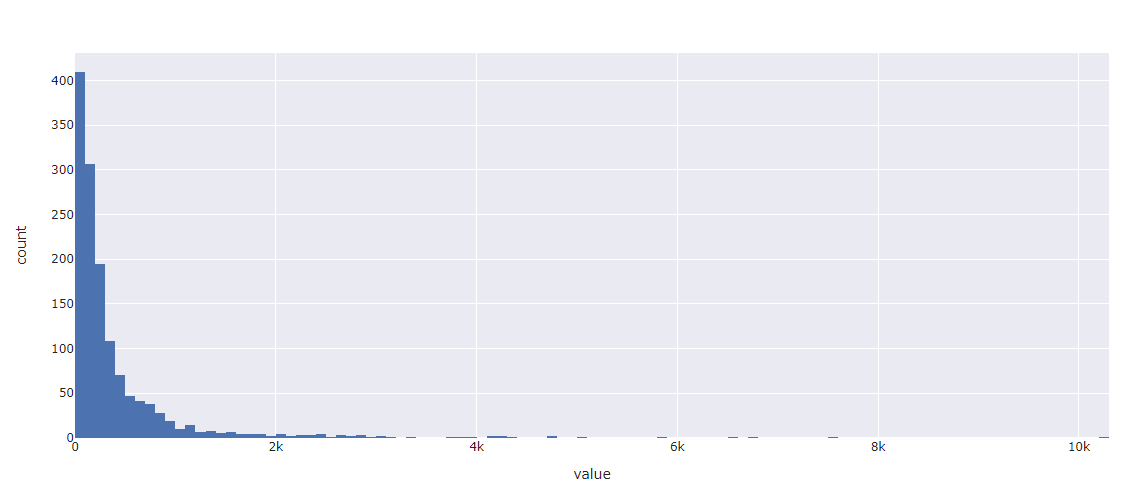
\includegraphics[width=\textwidth]{mean_rank_points}
\captionof{figure}{Mean rank points}
\label{fig:mean_rank_points}
\end{minipage}%
\begin{minipage}{.5\textwidth}
\centering
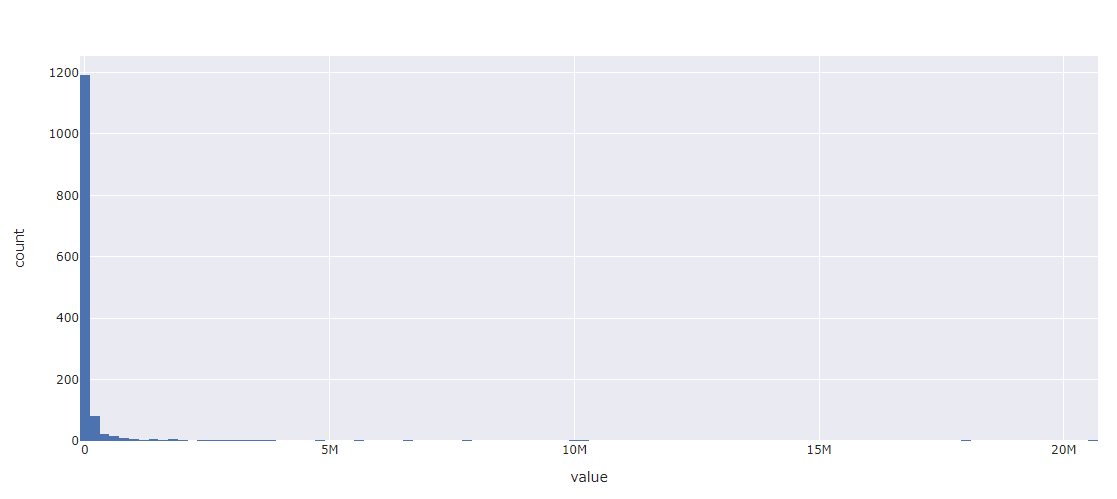
\includegraphics[width=\textwidth]{variance_rank_points}
\captionof{figure}{Variance rank points}
\label{fig:matches_per_year_and_month}
\end{minipage}
\begin{minipage}{.5\textwidth}
\centering
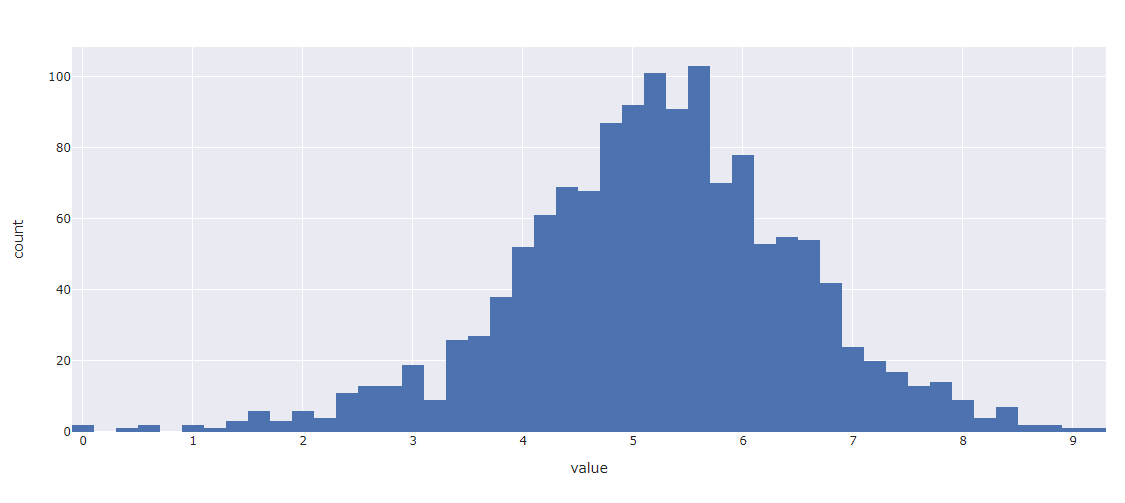
\includegraphics[width=235px]{log_mean_rank_points}
\captionof{figure}{Log mean rank points}
\label{fig:matches_per_day}
\end{minipage}%
\begin{minipage}{.5\textwidth}
\centering
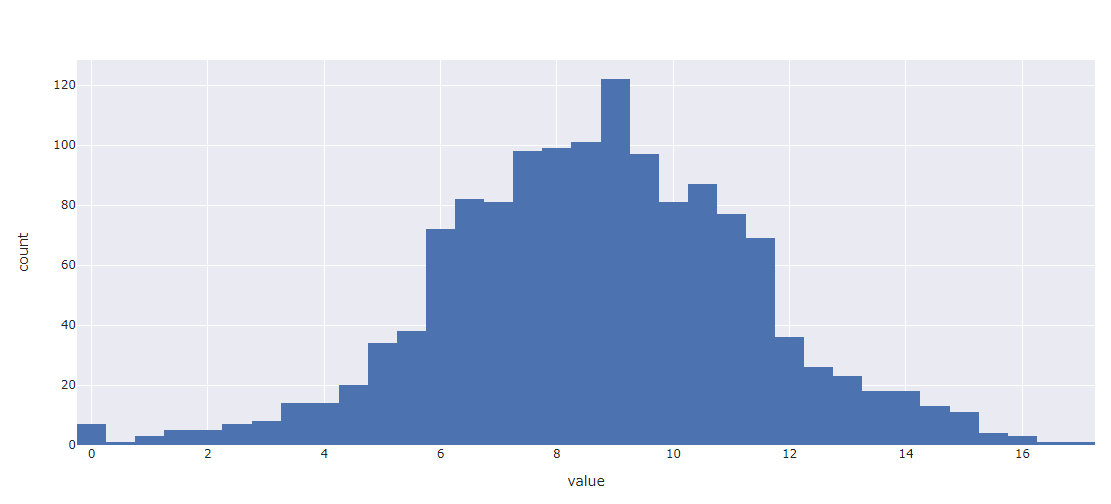
\includegraphics[width=235px]{log_variance_rank_points}
\captionof{figure}{Log variance rank points}
\label{fig:log_variance_rank_points}
\end{minipage}
\end{figure}

\subsubsection{Optimal K}
The optimal choice for k was done by following the elbow rule, that suggested to use $k=4$ where the SSE score was 96.214 (Fig. \ref{fig:kmeans_elbow_rule}). The clusters were fairly balanced and all of them crossed the Average Silhoutte Score of 0.44 (Fig. \ref{fig:kmeans_silhouette_score}). In other words, the closer it is to one, the better the object is matched to its own cluster and poorly matched to neighbouring clusters.


\begin{figure}[!h]
\centering
\begin{minipage}{.5\textwidth}
\centering
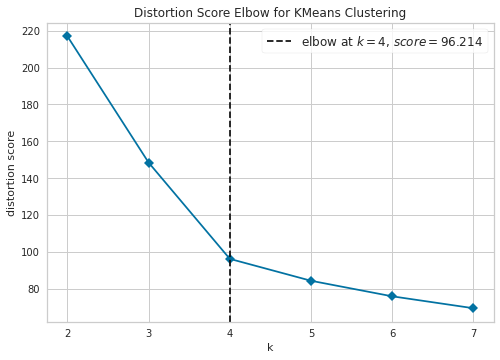
\includegraphics[width=\textwidth]{kmeans_elbow_rule}
\captionof{figure}{Elbow rule}
\label{fig:kmeans_elbow_rule}
\end{minipage}%
\begin{minipage}{.5\textwidth}
\centering
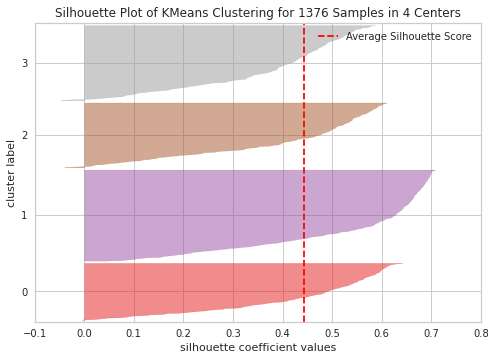
\includegraphics[width=\textwidth]{kmeans_silhouette_score}
\captionof{figure}{Silhouette score}
\label{fig:kmeans_silhouette_score}
\end{minipage}
\end{figure}

\subsubsection{Results interpretation}
Looking at the histograms (\ref{fig:total_match_played_kmeans}, \ref{fig:mean_rank_points_kmeans}, \ref{fig:age_kmeans}, \ref{fig:lrpOnAvgrp_kmeans}) we can interpret that:

\begin{itemize}
    \item{ \textbf{Cluster 1} represents the young promises: with good mean\_rank\_points, low age and a strong growth in ranking points.}
    \item{ \textbf{Cluster 0}: represents the declining strong players: older, with a good mean\_rank\_points but with a decreasing one.}
    \item{ \textbf{Cluster 2,3} represent the several worst players, divided in:}
    \begin{itemize}
        \item{2: older and declining player.}
        \item{3: older and slightly increasing in score.}
    \end{itemize}
\end{itemize}

%- forti, con un numero di match piu alti
%	- forti in declino e vecchi (e non prende gli outliers)
%	- forti in ascesa e giovani (promesse) con un gran numero match giocati
%- deboli, con un numero di match piu basso
%	- forte declino e piu vecchi
%	- forte ascesa e giovani
	
%	(Fig. \ref{fig:kmeans_results})
%	mean_rank_points, age, lrp_onAvgrp, total_matches_plyaed

\begin{figure}
\centering
\begin{minipage}{.5\textwidth}
\centering
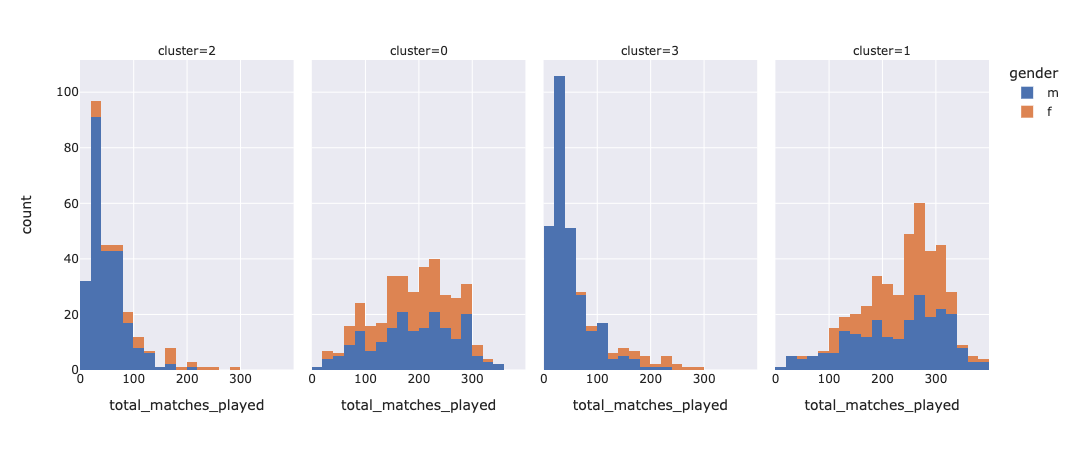
\includegraphics[width=\textwidth]{total_match_played_kmeans}
\captionof{figure}{total\_matches\_played histogram}
\label{fig:total_match_played_kmeans}
\end{minipage}%
\begin{minipage}{.5\textwidth}
\centering
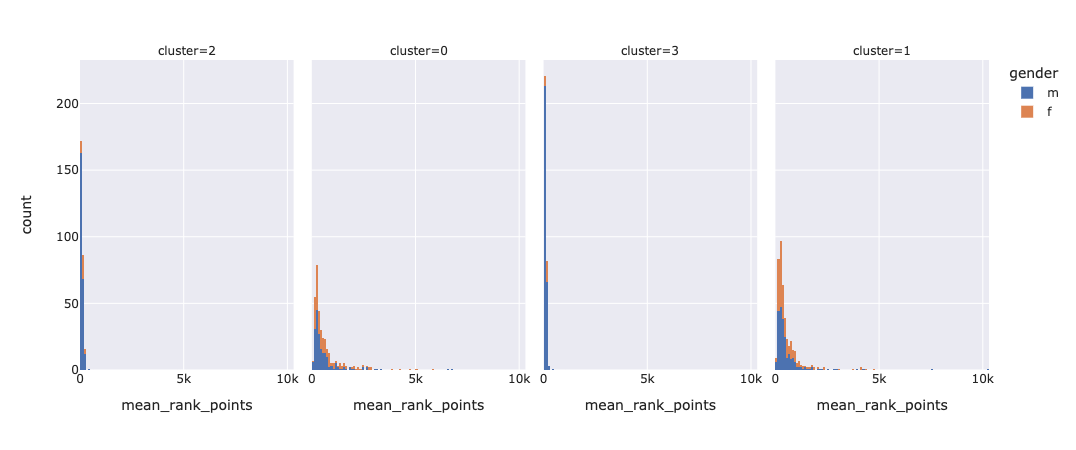
\includegraphics[width=\textwidth]{mean_rank_points_kmeans}
\captionof{figure}{mean\_rank\_points histogram}
\label{fig:mean_rank_points_kmeans}
\end{minipage}

\centering
\begin{minipage}{.5\textwidth}
\centering
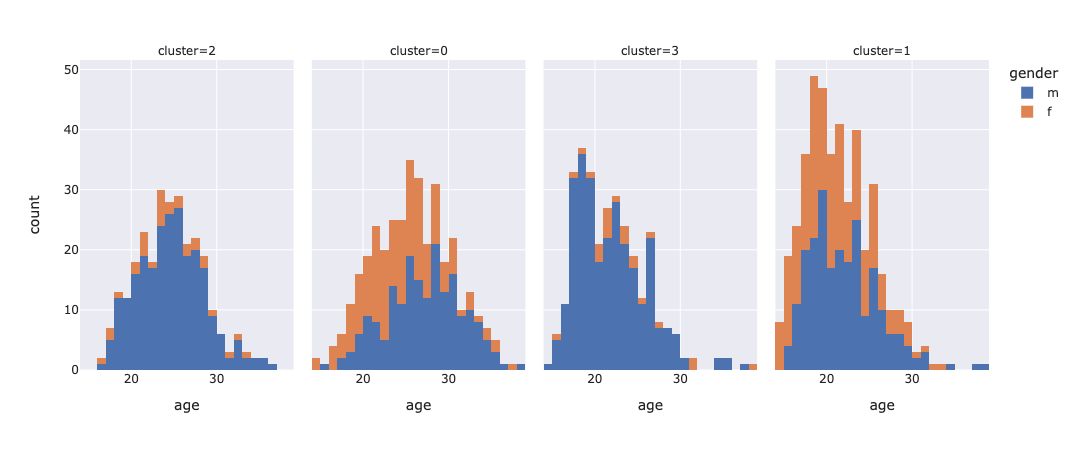
\includegraphics[width=\textwidth]{age_kmeans}
\captionof{figure}{age histogram}
\label{fig:age_kmeans}
\end{minipage}%
\begin{minipage}{.5\textwidth}
\centering
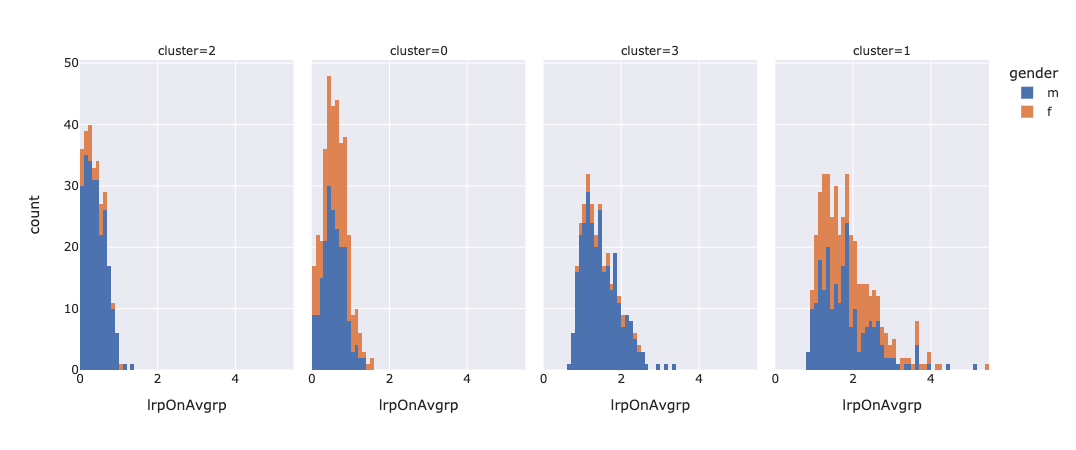
\includegraphics[width=\textwidth]{lrpOnAvgrp_kmeans}
\captionof{figure}{lrpOnAvgrp histogram}
\label{fig:lrpOnAvgrp_kmeans}
\end{minipage}
\end{figure}

\begin{figure}[h]
\centering
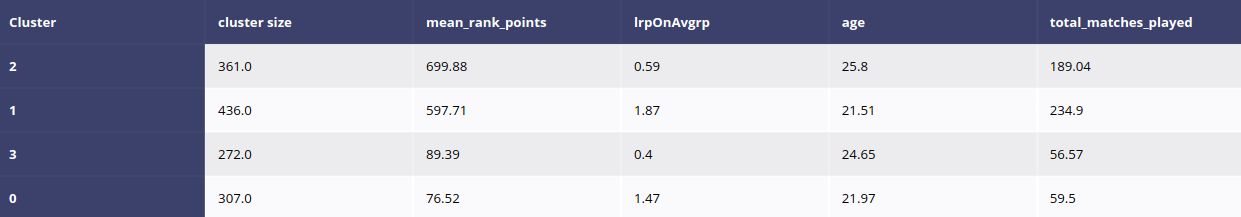
\includegraphics[width=.6\textwidth]{kmeans_results}
\captionof{figure}{Results of K-means}
\label{fig:kmeans_results}
\end{figure}

\newpage
\subsection{Density based}
The set of feature used for DBSCAN is the same as Kmeans. Here we opted to avoid the logarithm transformation and to use the StandardScaler rather than the MinMaxScaler, in order to give more weight to the good outliers that are an intrinsic characteristic of competitive games.\\
To understand a good range of values for eps we print the following plot \ref{fig:dbscan_distances} to check the distances between the k-th values for each point.

\begin{figure}[h]
\centering
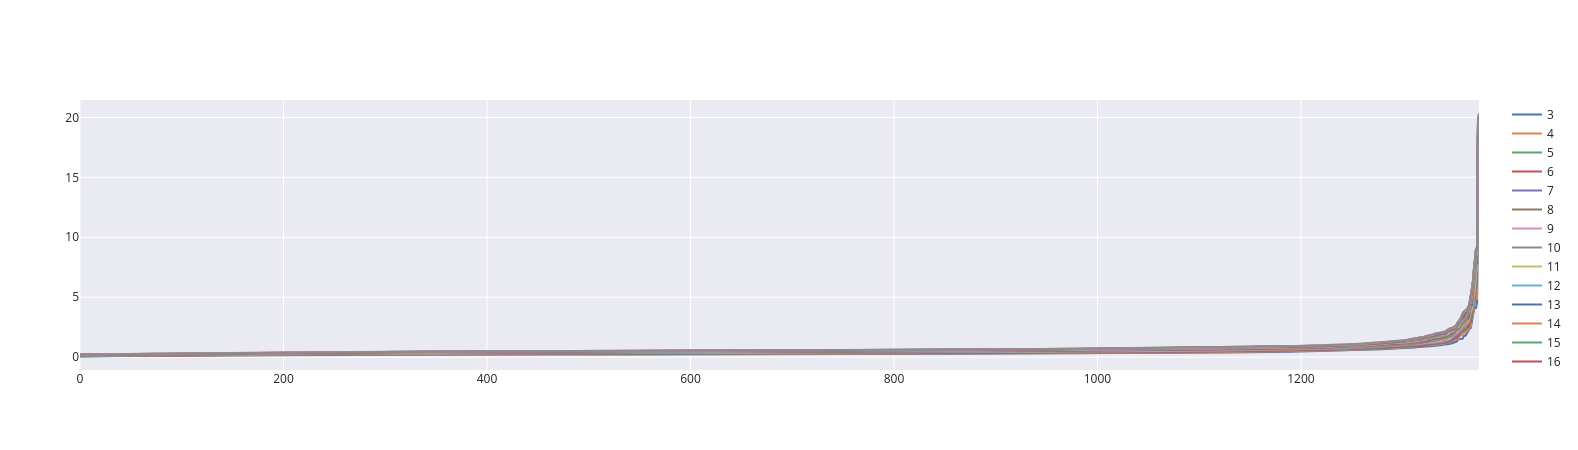
\includegraphics[width=\textwidth]{dbscan_distances}
\captionof{figure}{Noise points with the k-th nearest neighbor at farther distance}
\label{fig:dbscan_distances}
\end{figure}

Then we run a grid-search using as a range of values for eps = $[0.1, 2.9]$ \ref{fig:dbscan_metrics}. Through the grid search, we could get a better understanding of the kind of results we could expect for each rank and the resulting number of clusters.

\begin{figure}[h]
\centering
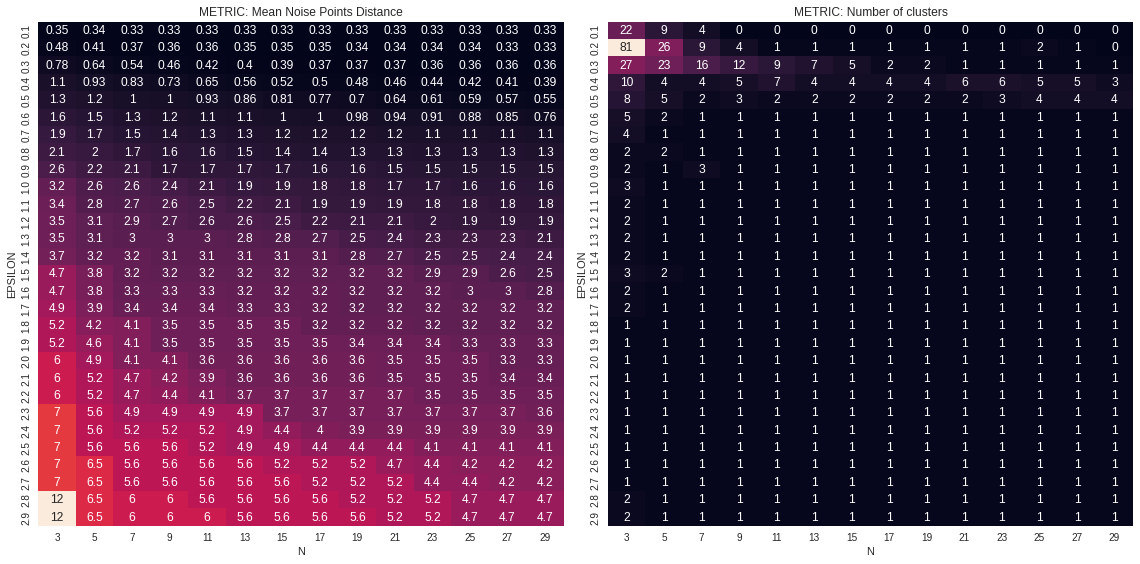
\includegraphics[width=.6\textwidth]{dbscan_metrics}
\captionof{figure}{Chosen hyper-parameters $eps=1$ and $n=3$}
\label{fig:dbscan_metrics}
\end{figure}

\subsubsection{Results interpretation}
The best combination of hyperparameters seemed to be $eps=1$ and $n=3$. The clusters result very unbalanced in the number of elements, probably the smaller clusters were very distant from the original distribution and this resulted in having clusters with very different characteristic from the single bigger cluster which characterise most of the players:

\begin{itemize}
\item \textbf{Cluster 1 , 2, -1}
    \begin{itemize}
        \item The promises (Cluster 1): Pretty strong ranking with extreme growth and very young.
	    \item Cluster 2: Strong players and pretty young
	    \item The veterans (Cluster -1), DBscan classified the outliers as the strongest players. The strongest, the oldest and with a growing score.
	 \end{itemize}
\item \textbf{Cluster 0}: The bigger cluster, relative to the remaining larger group
\end{itemize}	
	
\begin{figure}[h]
\centering
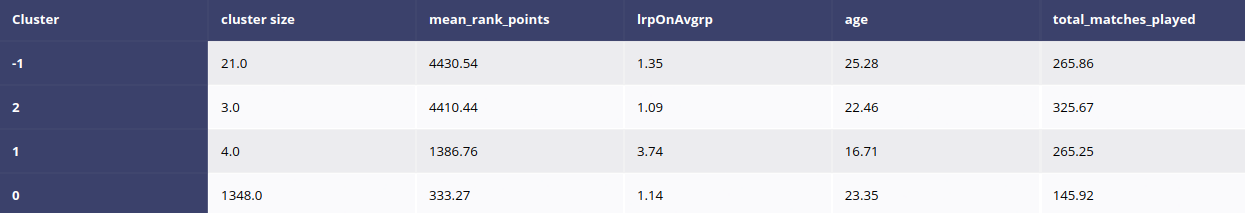
\includegraphics[width=.6\textwidth]{dbscan_results}
\captionof{figure}{Results of DBSCAN}
\label{fig:dbscan_results}
\end{figure}

\subsection{Hierarchical}
As in the DBSCAN we decided to go for a StandardScaler. The dendrogram used to create the cluster was created with a truncate mode $p=9$. The goal was to achieve a more in depth description of the players' profile. While the number of cluster was set to $k=7$ by using the WARD method for the linkage criterion.

\begin{figure}[h]
\centering
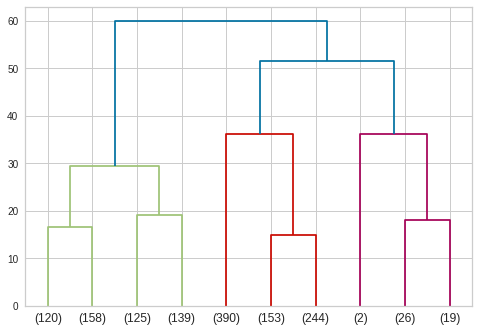
\includegraphics[width=.6\textwidth]{hierarchical_dendrogram}
\captionof{figure}{Results of Hierarchical}
\label{fig:hierarchical_dendrogram}
\end{figure}

\subsubsection{Results interpretation}
The hierarchical clustering subdivided the players in three principal clusters: strong, medium ability and weak players. Strong players were further divided in:
\begin{itemize}
    \item Extremely strong with a very high age and a high number of match played (medium-low last ranking points due to a single player).
    \item Strong on the rise. 
\end{itemize}
Medium ability players were further divided in:
\begin{itemize}
    \item On the rise and young.
    \item In descent and old. 
\end{itemize}
Weak players were further divided in:
\begin{itemize}
    \item In extreme descent and old.
    \item Young promises.
    \item Weak in general.
\end{itemize}
	
\begin{figure}[h]
\centering
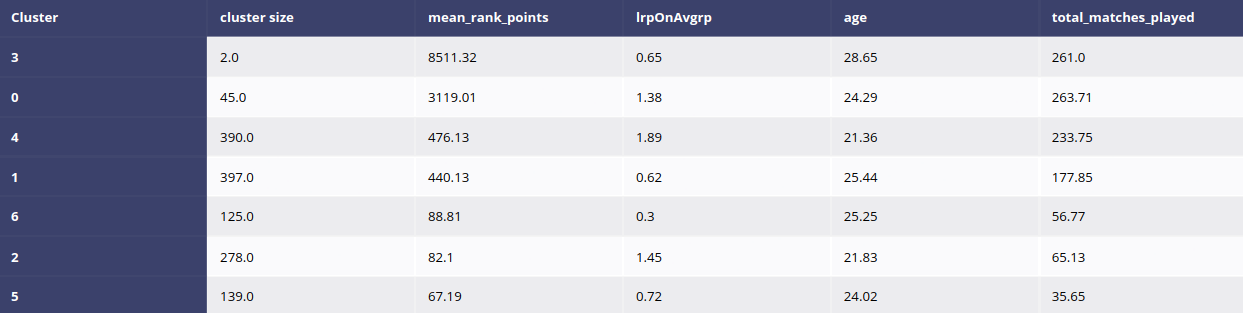
\includegraphics[width=.6\textwidth]{hierarchical_results}
\captionof{figure}{Results of Hierarchical}
\label{fig:hierarchical_results}
\end{figure}

\subsection{Gaussian Mixture}
For the current time being, we tried to exploit the Expectation-Maximization clustering algorithm for Gaussian Mixture Model (GMM) offered by the pyclustering library on the same initially selected features. The algorithm was initialized with a $k=5$ but the output was just $3$ clusters. In the results you can see a behaviour diametrically opposite to that of the DBSCAN, in fact this cluster is focused over the extreme weak players rather than describing with a better accuracy the strong players.  

\begin{itemize}
    \item{ \textbf{Cluster 1} is formed by 1360 players, and it's the biggest one. It's essentially a cluster that described the average profile of a player.}
    \item{ \textbf{Cluster 2} is a small group of 5 weak players that played few matches, but they are improving.}
    \item{\textbf{Cluster 0} is a small group of 11 weak players, but in this case they are younger, and they are not improving so much.}
\end{itemize}

\begin{figure}[h]
\centering
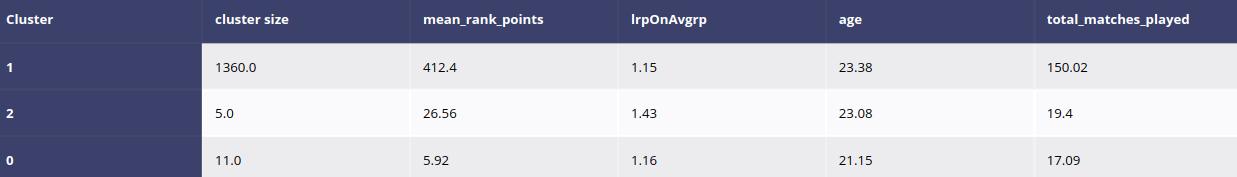
\includegraphics[width=.6\textwidth]{gm_results}
\captionof{figure}{Results of Gaussian Mixture}
\label{fig:gm_results}
\end{figure}

\subsection{Comparison}
Let's compare the different algorithms used and draw conclusions.

\begin{itemize}
    \item{ \textbf{K-means} identifies 4 very even distributions and manages to describe both fairly weak and fairly strong players. And for both it identifies those who are rising and those who are falling.  }
    \item{ \textbf{DBSCAN} is the one that identifies and describes in a better way the players that are excellent at tennis. But it does a poor job in describing all the others, that are just clustered in one huge group.}
    \item{\textbf{Hierarchical} is able to find fairly balanced groups and at the same time maintain a certain flexibility in order to be able to identify the very small group of formidable players. Moreover, it is able to group not only by strong and weak players, but also by intermediate players. In addition, for each group, it is able to identify those on the way up and those on the way down.}
    \item{\textbf{GM}} like DBSCAN but focuses on weak players.
\end{itemize}

In conclusion, the algorithm that manages to describe in the most detailed way the types of players within the dataset is without a doubt the Hierarchy.
\end{document}
